% !TEX root = tarasov-qasp-zh.tex
% 章首扉图与格言（sec-h）在英文源 ch-20.tex 尾部为 % 注释的死代码副本，非有效代码，未搬入；
% 本章文件首尾均无有效 sec 块。

\chapter[你对气体定律了解多少？]{你对气体定律了解多少？\label{ch-20}}

\begin{dialogue}

\tchr 请写出综合气体定律（combined gas law）的方程。

\stda 这个方程的形式是
\begin{equation}%
\frac{pV}{T} = \frac{p_{0}V_{0}}{T_{0}}
\label{eq-103}
\end{equation}
其中 $p$、$V$、$T$ 是一定质量的气体在某一状态下的压强、体积和温度，$p_{0}$、$V_{0}$、$T_{0}$ 是同一质量的气体在初始状态下的各对应量。温度以绝对温标表示。

\stdb 我更愿意用另一种形式的方程
\begin{equation}%
pV = \frac{m}{\mu} RT
\label{eq-104}
\end{equation}
其中 $m$ 是气体的质量，$\mu$ 是一个克分子的质量，$R$ 是普适气体常量（universal gas constant）。

\tchr 综合气体定律的这两种形式都是正确的。（对\smallcaps{学生乙}）你用到了普适气体常量。请讲讲，你怎样算出它的数值？我看这个值是背不下来的。
\pnote{式~\eqref{eq-103} 即 $pV/T=$~恒量，人教版选择性必修第三册第二章称理想气体状态方程，由“气体的等温变化”“气体的等压变化和等容变化”两节的三条实验定律导出；式~\eqref{eq-104} 即 $pV=nRT$，其中 $n=m/\mu$ 就是物质的量（原书的 $m/\mu$ 为克分子数，$\mu$ 为克分子量，数值等于现行记法的摩尔质量，g/mol）。$pV=nRT$ 通称克拉珀龙方程（Clapeyron equation），化学与大学普通物理中常用。}

\stdb 要计算 $R$，我可以用式~\eqref{eq-103}，其中参量 $p_{0}$、$V_{0}$、$T_{0}$ 属于同一质量的气体，只是取标准状况（standard conditions）下的数值。这就是说，$p_{0}= \SI{76}{\centi\meter}$~Hg（厘米汞柱），$T_{0}=\SI{273}{\kelvin}$，而 $V_{0} =\left( \dfrac{m}{\mu} \right) \times \SI{22.4}{\litre}$，因为在标准状况下，任何气体的一个克分子都占有确定的体积，等于 \SI{22.4}{\litre}。比值 $m/\mu$ 显然就是给定质量的气体中所含克分子的数目。把这些值代入式~\eqref{eq-103}，得
\begin{equation*}%
pV = \left( \frac{m}{\mu}\right) \, T \,\, \left( \frac{\SI{76}{\centi\meter} \,\,\text{Hg} \times \SI{22.4}{\litre}}{\SI{273}{\kelvin}} \right)
\end{equation*}
把它与表达式~\eqref{eq-104} 比较，便得 $R=6.2 \,(\si{\centi\meter}~\text{Hg}) \dfrac{\text{litres}}{\text{deg}}$。
\pnote{原书的 $R$ 值用的是厘米汞柱·升/度的混合单位。$1~\mathrm{cmHg}\approx 1333~\mathrm{Pa}$，故 $6.2~\mathrm{cmHg\cdot L/deg}\approx 8.3~\mathrm{J/(mol\cdot K)}$。现行值 $R=8.314~\mathrm{J/(mol\cdot K)}$（人教版取 8.31，称摩尔气体常量）；2019 年 SI 改革后 $N_{A}$、$k$ 均为定义值，$R=N_{A}k$ 随之为精确值 $8.314\,462\,618~\mathrm{J/(mol\cdot K)}$。原书的 $273~\mathrm{K}$、$22.4~\mathrm{L}$ 也是两位有效数字近似（现行 $273.15~\mathrm{K}$、$22.4~\mathrm{L/mol}$）；$76~\mathrm{cmHg}$ 即 $1$ 标准大气压 $101\,325~\mathrm{Pa}$。位数差异不影响任何中学结论。}

\tchr 我特意让你们做这些计算，为的是演示表达式~\eqref{eq-103} 与~\eqref{eq-104} 的等价性。遗憾的是，考生通常只知道式~\eqref{eq-103}，不熟悉式~\eqref{eq-104}，而后者与前面根据分子动理论考虑所得到的式~\eqref{eq-102} 完全一致。比较式~\eqref{eq-102} 与~\eqref{eq-104} 可得 $( m/\mu)R=Nk$。于是
\begin{equation}%
R=\frac{N}{\left( \dfrac{m}{\mu} \right)} k =N_{A}k
\label{eq-105}
\end{equation}
可见普适气体常量原来是阿伏加德罗常数与玻耳兹曼常量的乘积。接下来看看你们会不会使用综合气体定律的方程。\hlred{请用坐标轴 $V$ 和 $T$ 画出描述等压过程（isobaric process），即气体压强保持不变的过程的曲线。}

\stda 我似乎记得，这个过程由一条直线描述。

\tchr 为什么要靠回忆？用式~\eqref{eq-104} 嘛。以它为根据，把气体的体积表示成温度的函数。

\stda 由式~\eqref{eq-104} 得
\begin{equation}%
V = \left( \dfrac{m}{\mu} \right) \left( \dfrac{R}{p} \right) T
\label{eq-106}
\end{equation}
\tchr 这里的压强与温度有关吗？

\stda 在本题情形中无关，因为我们处理的是等压过程。

\tchr 好。那么式~\eqref{eq-106} 中的乘积 $\left( \dfrac{m}{\mu} \right) \left( \dfrac{R}{p} \right)$ 就是一个常量因子。这样我们就得到了气体体积对温度的线性依赖关系。考生通常能在以 $p$ 和 $V$ 为坐标轴的图上画出\hlred{等压}（$p$=const）、\textcolor{violet}{等温}（isothermal，$T$=const）和\hlblue{等容}（isochoric，$V$=const）过程；可是换成别的坐标轴组合，比如 $V$ 和 $T$ 或 $T$ 和 $p$，他们往往就画不出来了。\figr{fig-73} 中在不同的坐标系下画出了这三种过程。
\begin{figure*}
\centering
%\fbox{
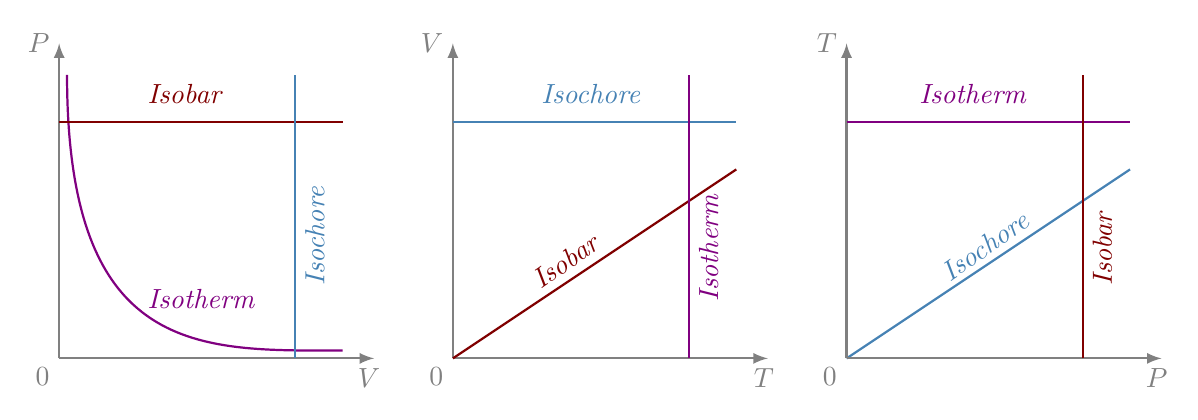
\begin{tikzpicture}
[>=latex,scale=2]
	
	\clip (-2.7,-0.21) rectangle (4.55, 2.1);
	%\draw[gray,step=0.2] (-3,-1) grid (5, 3);
	
	\node[below right,Maroon] at (-2,1.8 ) 
	{\emph{Isobar}};
	\node[below right,SteelBlue] at (.5,1.8 ) 
	{\emph{Isochore}};
	\node[below right,violet] at (2.9,1.8 ) 
	{\emph{Isotherm}};
	
	\node[below right,SteelBlue,rotate=90] at (-1,.4 ) 
	{\emph{Isochore}};
	\node[below right,violet,rotate=90] at (1.5,.3 ) 
	{\emph{Isotherm}};
	\node[below right,Maroon,rotate=90] at (4,.4 ) 
	{\emph{Isobar}};

	\node[below right,violet,] at (-2,.5 ) 
	{\emph{Isotherm}};
	\node[below right,Maroon,rotate=35] at (0.4,.55 ) 
	{\emph{Isobar}};
	\node[below right,SteelBlue,rotate=35] at (3,.6 ) 
	{\emph{Isochore}};
		
	\draw[thick, ->, gray] (0,0) -- (2,0);
	\draw[thick, ->, gray] (0,0) -- (0,2);

	\node [left,gray] at (-2.5,2) {$P$};
	\node [left,gray] at (0,2) {$V$};
	\node [left,gray] at (2.5,2) {$T$};
	
	\node [below left, gray] at (2.1,0) {$T$};
	\node [below left, gray] at (4.6,0) {$P$};
	\node [below left, gray] at (-.4,0) {$V$};
	
	\node [below left,gray] at (0,0) {0};
	\node [below left,gray] at (2.5,0) {0};
	\node [below left,gray] at (-2.5,0) {0};
	
	\draw[thick, violet] (-2.45,1.8) .. controls (-2.45,0) and (-1.6,.05) .. (-.7,.05);
	\draw[thick, SteelBlue] (2.5,0) -- (4.3,1.2);
	\draw[thick, Maroon] (0,0) -- (1.8,1.2);

	
	\draw[thick, ->, gray] (2.5,0) -- (4.5,0);
	\draw[thick, ->, gray] (2.5,0) -- (2.5,2);
	
	\draw[thick, ->, gray] (-2.5,0) -- (-.5,0);
	\draw[thick, ->, gray] (-2.5,0) -- (-2.5,2);
	
	\draw[thick, Maroon] (-2.5,1.5) -- (-.7,1.5);
	\draw[thick, SteelBlue] (0,1.5) -- (1.8,1.5);
	\draw[thick, violet] (2.5,1.5) -- (4.3,1.5);
	
	\draw[thick, SteelBlue] (-1,0) -- (-1,1.8);
	\draw[thick, violet] (1.5,0) -- (1.5,1.8);
	\draw[thick, Maroon] (4,0) -- (4,1.8);
\end{tikzpicture}%}
\caption[气体定律。]{气体定律。\label{fig-73}}
\end{figure*}

\stdb 关于 $V$、$T$ 坐标图中的等压线（isobar），我有一个问题。由式~\eqref{eq-106} 和\figr{fig-73} 中相应的曲线可见，当温度趋于零时，气体的体积也趋于零。可是，气体的体积无论如何也不可能小于它全部分子的体积总和。我的推理错在哪里？

\tchr 式~\eqref{eq-102}、\eqref{eq-103}、\eqref{eq-104} 和~\eqref{eq-106} 描述的都是所谓理想气体（ideal gas）。理想气体是真实气体的简化模型：它既不考虑分子的大小，也不考虑分子间的相互吸引。\figr{fig-73} 中的所有曲线都是对这种简化模型——即理想气体——而言的。

\stdb 可是气体定律与实验数据符合得很好，而实验中处理的是真实气体，它们的分子自有其大小。

\tchr 要注意，这类实验从来不在极低的温度下进行。只要真实气体没有被过度冷却或压缩，理想气体模型就能相当准确地描述它。还要注意，对空气中所含的气体（例如氮和氧）来说，在室温和通常压强下这些条件就已满足。

\stdb 您是说：如果对真实气体画出等压过程中体积对温度的依赖关系，那么在温度足够高时曲线与\figr{fig-73} 中相应的直线重合，而在低温区不再重合？

\tchr 正是。此外要记住，温度降得足够低时，气体会凝结成液体。

\stdb 我明白了。\figr{fig-73} 中式~\eqref{eq-106} 的曲线经过原点（零点）这一事实并无物理意义。那么，是否应当把曲线在到达这一点之前就截断呢？

\tchr 没有必要。你画的只是气体模型的曲线。至于这个模型适用于何处，那是另一个问题。现在我想提出下面的问题。\figr{fig-74} 在坐标轴 $V$ 和 $T$ 中画出了两条等压线：一条对应压强 $p_{1}$，另一条对应压强 $p_{2}$。哪个压强更高？

\stda 多半是 $p_{2}$ 高于 $p_{1}$。

\begin{figure}[!h]%
\centering
%\fbox{
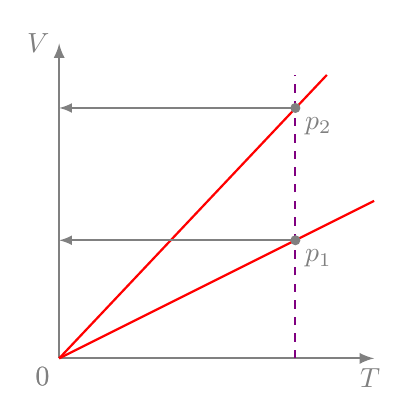
\begin{tikzpicture}	[>=latex ,scale=2]
	
	\clip (-.2,-0.21) rectangle (2.1, 2.1);
	%\draw[gray,step=0.2] (-3,-1) grid (5, 3);
		
	%\draw[thick,red] plot (\x,\x*\x)	;
	%\draw[thick,cyan] plot (\x,\x*\x*\x);
	
	%\node[below right,cyan] at (.5,1.8 ) 
	%{\emph{Isochore}};
	
	%\node[below right,violet,rotate=90] at (1.5,.3 ) 
	%{\emph{Isotherm}};
		
	\draw[thick, ->, gray] (0,0) -- (2,0);
	\draw[thick, ->, gray] (0,0) -- (0,2);
	\draw[thick, violet, dashed] (1.5,0) -- (1.5,1.8);

	\node [left,gray] at (0,2) {$V$};
	\node [below left, gray] at (2.1,0) {$T$};
	\node [below left,gray] at (0,0) {0};
	\node [below left,gray] at (0,0) {0};
	\node [below right,gray] at (1.5,.75) {$p_{1}$};
	\node [below right,gray] at (1.5,1.59) {$p_{2}$};
	
	\draw[thick, red] (0,0) -- (2,1);
	\draw[thick, red] (0,0) -- (1.7,1.8);
	\draw[<-,semithick,gray] (0,1.59) -- (1.5,1.59);
	\draw [fill,gray](1.5,1.59) circle (0.8pt);
	\draw[<-,semithick,gray] (0,.75) -- (1.5,.75);
	\draw [fill,gray](1.5,.75) circle (0.8pt);
\end{tikzpicture}%}
\caption[哪个压强更高？]{哪个压强更高？\label{fig-74}}
\end{figure}

\tchr 你不动脑筋就回答了。显然，你是这样想的：那条等压线更陡，对应的压强就更高。这完全错了。按照式~\eqref{eq-106}，等压线倾角的正切等于 $\left( \dfrac{m}{\mu} \right) \left( \dfrac{R}{p} \right)$。由此可见，压强越高，等压线的倾角越小。因此，在我们的情形里，$p_{2} < p_{1}$。用另一种推理也能得出同样的结论。我们在\figr{fig-74} 中画一条等温线（见虚线）。它与等压线 $p_{2}$ 的交点所对应的气体体积，大于与等压线 $p_{1}$ 的交点所对应的体积。我们知道，温度相同时，气体的体积越小，压强越高。这直接由综合气体定律得出［见式~\eqref{eq-103} 或~\eqref{eq-104}］。所以 $p_{2} < p_{1}$。

\stda 现在我确实懂了。

\tchr 那么请看\figr{fig-75}，其中画出了同一质量的气体在两个不同温度 $T_{1}$、$T_{2}$ 下的两条等温线（坐标轴为 $p$ 和 $V$）。哪个温度更高？

\begin{figure}[!h]%
\centering
%\fbox{
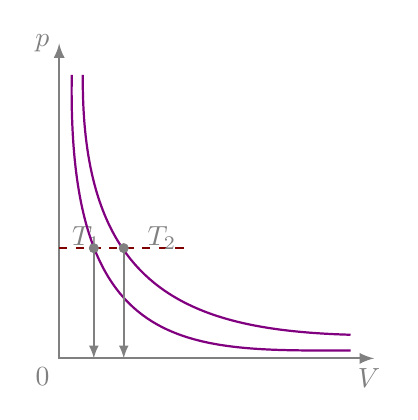
\begin{tikzpicture}[>=latex,scale=2]
	
	\clip (-.2,-0.21) rectangle (2.1, 2.1);		
	\draw[thick, <->, gray] (2,0) -- (0,0) -- (0,2);
	\draw[thick, Maroon, dashed] (0,0.7) -- (.8,0.7);
	\node [left,gray] at (0,2) {$p$};
	\node [below left, gray] at (2.1,0) {$V$};
	\node [below left,gray] at (0,0) {0};
	\node [below right,gray] at (.02,.9) {$T_{1}$};
	\node [below right,gray] at (.5,.9) {$T_{2}$};
	\draw[ thick, violet] (.08,1.8) .. controls (.05,.01) and (.8,.05) .. (1.85,.05);
	\draw[ thick, violet] (.15,1.8) .. controls (.14,.45) and (.8,.18) .. (1.85,.15);
	\draw[->,semithick,gray] (0.22,.7) -- (0.22,0);
	\draw [fill,gray](0.22,.7) circle (0.8pt);
	\draw[->,semithick,gray] (0.41,.7) -- (0.41,0);
	\draw [fill,gray](0.41,.7) circle (0.8pt);

\end{tikzpicture}%}
\caption[哪个温度更高？]{哪个温度更高？\label{fig-75}}
\end{figure}
\pnote{底本图 75 的图题误沿图 74（同为“Which pressure is higher?”），而正文提问与本图内容（$p$--$V$ 坐标中的两条等温线 $T_{1}$、$T_{2}$，以及比较同一压强下体积的等压虚线）问的都是“哪个温度更高”，显系录入误抄；中文版按图面与上下文拟写图题，待考原书。}

\stda 我先画一条等压线（\figr{fig-75} 中的虚线（\begin{tikzpicture}\draw[thick, Maroon, dashed] (0,0) -- (.4,0);\end{tikzpicture}））。压强不变时，气体温度越高，体积越大。因此，最外面的等温线 $T_{2}$ 对应较高的温度。

\tchr 对。请记住：在 $p$、$V$ 坐标中，等温线离原点越近，温度越低。

\stdb 我们中学里学气体定律的范围比现在的讨论窄得多。综合气体定律只是勉强提了一下，所学仅限于玻意耳--马略特定律、盖-吕萨克定律和查理定律。

\tchr 对此，我想作几点说明，使玻意耳--马略特定律、盖-吕萨克定律和查理定律都能纳入总的图景。玻意耳--马略特定律（更常称为玻意耳定律）描述等温过程中 $p$ 与 $V$ 的关系。它的方程形式是
\begin{equation}%
p=\frac{\text{constant}}{V}
\label{eq-107}
\end{equation}
式中常量 $\text{constant}= \left( \dfrac{m}{\mu} \right) RT$。

盖-吕萨克定律描述等容过程中 $p$ 与 $T$ 的关系。它的方程是
\begin{equation}%
p=\text{constant} \,\,T
\label{eq-108}
\end{equation}
式中常量 $\text{constant}= \left( \dfrac{m}{\mu} \right) \dfrac{R}{V}$。

查理定律描述等压过程中 $V$ 与 $T$ 的关系。它的方程是
\begin{equation}%
V=\text{constant} \,\,T
\label{eq-109}
\end{equation}
式中常量 $\text{constant}= \left( \dfrac{m}{\mu} \right) \dfrac{R}{p}$。［式~\eqref{eq-109} 显然与式~\eqref{eq-106} 重复。］对上述各条气体定律，我要作以下几点说明：
\pnote{注意命名传统：本书英文本按英美习惯，把等容过程中 $p\propto T$ 的定律（式~\eqref{eq-108}）称为盖-吕萨克定律，把等压过程中 $V\propto T$ 的定律（式~\eqref{eq-109}）称为查理定律；我国教材（承俄、法等国传统）恰好相反——人教版选择性必修第三册第二章第 3 节“气体的等压变化和等容变化”中，查理定律指等容变化（$p/T=$~恒量），盖-吕萨克定律指等压变化（$V/T=$~恒量）。分歧源于史料：查理 1787 年的研究未发表，盖-吕萨克 1802 年发表时一并引用。中文版照译原书命名，读者按内容对号即可。玻意耳定律（马略特独立发现同一规律）即人教版该章第 2 节“气体的等温变化”。}
\begin{enumerate}[label=(\arabic*),leftmargin=1cm]
\item 所有这些定律都是对理想气体而言的；对真实气体，只在理想气体模型能描述它的范围内适用。
\item 每条定律都在假定第三个参量保持不变的条件下，建立气体某两个参量之间的关系。
\item 容易看出，每条定律都是综合气体定律［见式~(\ref{eq-104})］的推论；后者建立三个参量之间的关系，不附有任何特殊条件。
\item 这些定律中的常量，可以不用气体质量和保持恒定的第三个参量来表示，而用同一质量的气体在另一状态下的同一对参量来表示。换句话说，气体定律可以改写成下列形式
\begin{align}%
p & = \frac{p_{0}V_{0}}{V} \tag{107a} \label{107a} \\
p & = \frac{p_{0}}{T_{0}} T \tag{108a}\label{108a} \\
V & = \frac{V_{0}}{T_{0}} T \tag{109a} \label{109a}
\end{align}
\end{enumerate}
\stda 看来我终于弄懂气体定律的实质了。

\tchr 那就继续往下讲。看下面这个例子。\hlred{气体以这样的方式膨胀：它的压强和体积满足条件}
\begin{equation}%
\hlred{pV^{2} = \text{constant}}
\label{eq-110}
\end{equation}
\hlred{要弄清楚：在这样的膨胀中，气体是被加热了，还是相反，被冷却了。}

\stda 为什么气体的温度一定会变化呢？

\begin{figure}[!h]%
\centering
\includegraphics[width=0.4\textwidth]{figs/ch-20/fig-076a}
\caption[两条曲线的比较。]{比较 $p \propto \dfrac{1}{V^{2}}$ 与 $p \propto \dfrac{1}{V}$ 的两条曲线。\label{fig-76}}
\end{figure}
\pnote{底本图题把两条曲线称为 isochores（等容线），但本图与所附原书扫描图都是 $p$--$V$ 坐标：$p\propto 1/V$ 是玻意耳等温线，$p\propto 1/V^{2}$ 是题给的过程曲线，学生下文也说“过渡到越来越靠近原点的等温线”。等容线在 $p$--$V$ 图中应是竖直线，故“等容线”显系笔误，中文版径改译“曲线”，待考原书。}

\tchr 如果温度保持不变，那就意味着气体按玻意耳--马略特定律［式~\eqref{eq-107}］膨胀。等温过程中 $p \propto \dfrac{1}{V}$，而我们的情形里 $p$ 对 $V$ 的依赖关系性质不同：$p \propto \dfrac{1}{V^{2}}$。

\stda 也许我可以试着把这些关系画成图？曲线的形状就如\figr{fig-76} 所示。

\tchr 这个想法好。这些曲线说明什么？

\stda 我现在似乎明白了。可以看到，沿着曲线 $p \propto \dfrac{1}{V^{2}}$ 向体积增大的方向走，气体会逐渐过渡到离原点越来越近的等温线上，也就是对应于温度不断降低的等温线。这就是说，在这个膨胀过程中气体被冷却。

\tchr 完全正确。只是我要把你的答案换个说法：这样的气体膨胀过程，只有在气体同时被冷却的条件下才可能进行。

\stdb 这个结论能用解析方法得到吗？

\tchr 当然可以。考虑气体的两个状态：$p_{1}, \,V_{1}, \,T_{1}$ 和 $p_{2},\, V_{2},\, T_{2}$。对每个状态写出综合气体定律［见式~\eqref{eq-104}］
\begin{align*}%
p_{1} V_{1} & = \frac{m}{\mu} RT_{1}\\
p_{2}V_{2} & = \frac{m}{\mu} RT_{2}
\end{align*}
按题设条件，给定的气体膨胀过程可以写成
\begin{equation*}%
p_{1} V_{1}^{2} = p_{2}V_{2}^{2}
\end{equation*}
把前面两个气体定律方程代入最后这个方程，得
\begin{equation*}%
\frac{m}{\mu} R T_{1} V_{1} = \frac{m}{\mu} R T_{2}V_{2}
\end{equation*}
约去公因子后得
\begin{equation}
T_{1} V_{1} = T_{2}V_{2}
\label{eq-111}
\end{equation}
由这个方程显然可见：比如气体的体积增大到两倍，它的温度（绝对温标的温度）就应当降低到一半。

\stda 这是不是说，不论气体经历什么过程，在每一瞬间它的参量（$p$、$V$ 和 $T$）都由综合气体定律相联系？

\begin{figure}[!h]%
\centering
\includegraphics[width=0.4\textwidth]{figs/ch-20/fig-077a}
\caption[气体做的功。]{气体做的功。\label{fig-77}}
\end{figure}
\tchr 正是这样。综合气体定律建立气体参量间的关系，不附任何条件。现在来考察在各种过程中气体与周围介质交换能量的性质。设气体正在膨胀。它会把限制其体积的所有物体都推回去（例如汽缸中的活塞）。于是，气体对这些物体做功。等压膨胀时气体做的功不难计算。设气体等压膨胀，把横截面积为 $S$ 的活塞推开一段距离 $\Delta l$（\figr{fig-77}）。气体作用在活塞上的压强为 $p$。求气体移动活塞所做的功：
\begin{equation}%
A = F \Delta l = (pS) \Delta l = p (S \Delta l) = p(V_{2} - V_{1})
\label{eq-112}
\end{equation}
其中 $V_{1}$ 和 $V_{2}$ 是气体初、末状态的体积。
\pnote{“不附任何条件”宜加一句限定：只有当气体所经历的每个中间态都近似为平衡态（准静态过程）时，才谈得上每一瞬间都有统一的 $p$、$V$、$T$ 并满足状态方程；急速膨胀等非平衡过程中，气体内部没有单一确定的压强。中学问题与考题默认准静态过程。}

非等压膨胀中气体所做的功计算起来要难一些，因为膨胀过程中压强在不断变化。一般情形下，气体体积从 $V_{1}$ 增大到 $V_{2}$ 所做的功，等于 $p(V)$ 曲线在 $V_{1}$ 与 $V_{2}$ 之间下方的面积。气体从体积 $V_{1}$ 等压地和等温地膨胀到体积 $V_{2}$ 所做的功，在\figr{fig-78} 中分别由全部画有斜阴影线的面积和画有交叉阴影线的面积表示；两种情形中气体的初态相同。可见，气体膨胀时对外界物体做功，是以自身的一部分内能为代价的。气体所做的功与膨胀过程的性质有关。还要注意，如果气体被压缩，那就是外界对气体做功，因而它的内能增大。
\pnote{“以一部分内能为代价做功”与“压缩则内能增大”，都是对气体与外界不交换热量（绝热）的情形说的：绝热膨胀内能减小，绝热压缩内能增大。等温膨胀时对外做的功全部来自吸收的热量，内能并不减小——这正是下面几段引入第二种能量交换方式（传热）的动机。}

\begin{figure}[!h]%
\centering
\includegraphics[width=0.4\textwidth]{figs/ch-20/fig-078a}
\caption[气体做的功。]{气体做的功。\label{fig-78}}
\end{figure}
\pnote{“$p$--$V$ 图像下的面积等于气体做的功”是高考与竞赛的常规工具：等压过程为矩形 $p(V_{2}-V_{1})$，一般过程为曲线下面积（大学写作 $\int p\,\mathrm{d}V$）。循环过程中的净功等于循环所围的面积，\figr{fig-79} 的循环即是一例。}

然而，做功并不是气体与介质交换能量的唯一方式。例如，等温膨胀中气体做了若干功 $A$，因而损失了等于 $A$ 的能量。可是另一方面，正如\chap{ch-18} 中所列各条原理所要求的那样［见式~\eqref{eq-98}］，等温过程中气体温度恒定，就意味着它的内能 $U$ 保持不变（我提醒一下：$U$ 由分子的热运动决定，而分子的平均能量与温度 $T$ 成正比）。问题是：在这种情形里，做功消耗的是什么能量？

\stdb 显然是从外界传给气体的热量。

\tchr 对。这样我们就得出结论：气体至少通过两条途径与介质交换能量：做与气体体积变化相联系的功，以及传热。能量平衡可以写成如下形式
\begin{equation}%
\Delta U = Q - A
\label{eq-113}
\end{equation}
其中 $\Delta U$ 是气体内能的增量（由气体温度的升高来表征），$Q$ 是从周围介质传给气体的热量，$A$ 是气体对周围物体所做的功。式~\eqref{eq-113} 称为热力学第一定律（first law of thermodynamics）。注意，它是普适的：不仅适用于气体，也适用于任何其他物体。
\pnote{注意符号约定：式~\eqref{eq-113} 中 $A$ 是气体对外界做的功。人教版选择性必修第三册第三章（第 1 节“功、热和内能的改变”、第 2 节“热力学第一定律”）取 $W$ 为外界对物体做的功，写作 $\Delta U=W+Q$（即 $W=-A$），并约定吸热 $Q>0$、外界做正功 $W>0$。两套写法完全等价，解题时务必先认清所用约定。}

\stdb 总结起来，我们可以得出结论：等温膨胀中，传给气体的热量全部立即转变为气体所做的功。如果是这样，那么等温过程就不可能在与外界热绝缘（绝热）的系统内发生。

\tchr 完全正确。现在从能量的角度考察气体的等压膨胀。

\stdb 气体膨胀，这意味着它在做功。同时，由式~\eqref{eq-106} 可见，气体的温度升高，也就是说它的内能增大。因此，这种情形下必须传给气体较多的热量：其中一部分用来增加气体的内能，其余的转变为气体所做的功。

\tchr 很好。再看一个例子。给气体加热，使它的温度升高 $\Delta T$。这样做两次：一次在气体体积不变的条件下，一次在压强不变的条件下。两种情形下消耗的热量相同吗？

\stda 我认为是的。

\stdb 我认为需要的热量不同。体积不变时气体不做功，全部热量都用于增加气体的内能，即升高它的温度。这时
\begin{equation}%
Q_{1} = C_{1} \Delta T
\label{114}
\end{equation}
压强不变时，加热必然伴随气体的膨胀，所做的功为 $A=p(V-V_{1})$。供给的热量 $Q_{2}$ 一部分用于增加气体的内能（升高温度），一部分用于做这份功。于是
\begin{equation}%
Q_{2} = C_{1} \Delta T + p(V-V_{1})
\label{eq-115}
\end{equation}
显然，$Q_{1} < Q_{2}$。

\tchr 我同意学生乙的看法。使物体的温度升高 1 度所需要的热量，你们把它叫作什么？

\stdb 物体的热容（heat capacity）。

\tchr 从上面这个例子能就气体的热容得出什么结论？

\stdb 气体有两种不同的热容：定容热容和定压热容。定容热容（即前两个方程中的因子 $C_{1}$）小于定压热容。

\tchr 你能把定压热容用 $C_{1}$（即定容热容）表示出来吗？

\stdb 我来试试。把定压热容记作 $C_{2}$。按照热容的定义，可以写 $C_{2}= Q_{2}/ \Delta T$。把式~\eqref{eq-115} 中 $Q_{2}$ 的值代入，得
\begin{equation}%
C_{2} = C_{1} + \frac{p(V-V_{1})}{\Delta T} 
\label{eq-116}
\end{equation}

\tchr 你停得太早了。运用综合气体定律的方程，可以写出
\begin{equation*}%
p(V-V_{1}) = \frac{m}{\mu} R (T - T_{1}) =  \frac{m}{\mu} R \Delta T
\end{equation*}
代入式~(\ref{eq-116}) 后，得
\begin{equation}%
C_{2} = C_{1} + \frac{m}{\mu} R
\label{eq-117}
\end{equation}
对气体的一个克分子（$m=\mu$）而言，这个关系更为简单：
\begin{equation}%
C_{2} = C_{1} + R
\label{eq-118}
\end{equation}
\pnote{$C_{1}$、$C_{2}$ 即定容热容与定压热容，大学物理记作 $C_{V}$、$C_{p}$（此处对整团气体而言，是总热容；中学教材的比热容按单位质量定义）。式~\eqref{eq-118} 即迈耶公式 $C_{p}-C_{V}=R$（对 1 mol 而言），中学不作要求；它把上文“升高同样温度时等压过程要多吸热以对外做功”定量化。延伸：由大学普通物理的能量均分定理还可得单原子理想气体 $C_{V}=\tfrac{3}{2}R$、双原子分子气体 $C_{V}=\tfrac{5}{2}R$。}

最后，考察某个由一条等温线、一条等容线（isochore）和一条等压线组成的循环（cycle）（见\figr{fig-79}~\drkgry{(a)}，其中以 $p$ 和 $V$ 为坐标轴）。请把同一个循环（定性地）画在以 $V$ 和 $T$ 为坐标轴的图上，并分析循环各段中气体与介质交换能量的性质。
\begin{figure}[!h]%
\centering
\includegraphics[width=0.4\textwidth]{figs/ch-20/fig-079a}
\caption[同一循环在两套坐标轴下的图形。]{同一循环在两套坐标轴下的图形：(a) 以 $p$、$V$ 为坐标轴；(b) 以 $V$、$T$ 为坐标轴。\label{fig-79}}
\end{figure}
\pnote{底本图 79 的图题误沿图 77、78（“Work done by a gas.”），本图实为同一循环在两套坐标轴下的图形：(a) $p$--$V$ 坐标，1--2 等温膨胀、2--3 等容升压、3--1 等压压缩；(b) $V$--$T$ 坐标。中文版按图面与正文拟写图题，待考原书。}

\stdb 在以 $V$ 和 $T$ 为坐标轴的图上，循环的形状如\figr{fig-79}~\drkgry{(b)} 所示。

\tchr 完全正确。现在请分析循环各段中气体与介质交换能量的性质。

\stdb 在 1--2 段，气体经历等温膨胀。它从外界吸收一定的热量，并把全部热量用于做功。气体的内能保持不变。

在循环的 2--3 段，气体被等容加热（体积不变）。由于体积不变，不做功。气体内能的增加仅仅依靠从外界传入的热量。

在 3--1 段，气体被等压压缩（压强不变），如\figr{fig-79}~\drkgry{(b)} 所示，它的温度下降。外界对气体做功，而它的内能却在减少。这意味着气体在强烈地向介质放热。

\tchr 你的推理完全正确。

\stda 这场讨论使我明白，我对气体定律知道得太少了。这一切都是入学考试所必须掌握的吗？依我看，我们讨论的有些问题已经超出了考生应考的物理大纲的范围。

\tchr 如果你仔细回想我们的讨论，就会看到它涉及的只是与综合气体定律（一般形式或应用于特殊情形）直接相关的问题。\hlblue{你的困惑不应归咎于大纲被凭空拉大了，而只能归咎于你还没有把气体定律反复思考、透彻理解。}遗憾的是，考生常常满足于对气体定律的一点极肤浅的认识，不肯再深入一步。

\end{dialogue}


\cleardoublepage

% NEWTERMS: combined gas law | 综合气体定律 | 即 pV/T=恒量；人教版选必三称理想气体状态方程；式 (104) 即克拉珀龙方程 pV=nRT
% NEWTERMS: universal gas constant | 普适气体常量 | 人教版称摩尔气体常量 R=8.31 J/(mol·K)；原书混合单位换算见评注
% NEWTERMS: isobaric process / isobar | 等压过程／等压线 | |
% NEWTERMS: isothermal process / isotherm | 等温过程／等温线 | |
% NEWTERMS: isochoric process / isochore | 等容过程／等容线 | 人教版选必三用“等容变化”
% NEWTERMS: ideal gas | 理想气体 | 正文首现于本章（ch-18 评注已提及）
% NEWTERMS: standard conditions | 标准状况 | 0 °C、1 atm；1 克分子气体占 22.4 L
% NEWTERMS: work done by the gas | 气体（对外）做的功 | 原书符号约定 A；与人教版 W 反号，见评注
% NEWTERMS: first law of thermodynamics | 热力学第一定律 | 人教版选必三第三章；符号约定差异见评注
% NEWTERMS: heat capacity | 热容 | 对整团气体计；按单位质量定义的是比热容
% NEWTERMS: heat capacity at constant volume / at constant pressure | 定容热容／定压热容 | 即 C_V、C_p；迈耶公式见评注
% NEWTERMS: cycle | 循环 | 各段（element）译“段”
% NEWTERMS: thermally insulated system | 热绝缘系统 | 即绝热系统
% NEWTERMS: Boyle and Mariotte's law / Boyle's law | 玻意耳--马略特定律／玻意耳定律 | 马略特独立发现；人教版选必三第二章第 2 节“气体的等温变化”
% NEWTERMS: Gay-Lussac's law | 盖-吕萨克定律 | 命名传统差异：本书（英美习惯）指等容 p–T 定律；人教版指等压 V–T 定律，见评注
% NEWTERMS: Charles' law | 查理定律 | 与上条相反：本书指等压 V–T 定律；人教版指等容 p–T 定律，见评注
% NEWTERMS: internal energy increment | 内能增量 | ΔU；术语承 ch-18“内能”
